\documentclass[a5paper]{article}
\usepackage[utf8]{inputenc}
\usepackage[IL2]{fontenc}
\usepackage{geometry}
\usepackage{tikz}
\usepackage{enumitem}
\graphicspath{ {img/} }
\usepackage[czech]{babel}

%%%%%%%%%%%%%%%%%%%%%%%%%%%%%%%%%%%%%%%%%%%%%%%%%%%%%%%%%%%%%%%%%%%%%%
% LaTeX Overlay Generator - Annotated Figures v0.0.1
% Created with http://ff.cx/latex-overlay-generator/
% If this generator saves you time, consider donating 5,- EUR! :-)
%%%%%%%%%%%%%%%%%%%%%%%%%%%%%%%%%%%%%%%%%%%%%%%%%%%%%%%%%%%%%%%%%%%%%%
%\annotatedFigureBoxCustom{bottom-left}{top-right}{label}{label-position}{box-color}{label-color}{border-color}{text-color}
\newcommand*\annotatedFigureBoxCustom[8]{\draw[#5,thick,rounded corners] (#1) rectangle (#2);\node at (#4) [fill=#6,thick,shape=circle,draw=#7,inner sep=2pt,font=\sffamily,text=#8] {\textbf{#3}};}
%\annotatedFigureBox{bottom-left}{top-right}{label}{label-position}
\newcommand*\annotatedFigureBox[4]{\annotatedFigureBoxCustom{#1}{#2}{#3}{#4}{red}{white}{black}{black}}
\newcommand*\annotatedFigureText[4]{\node[draw=none, anchor=south west, text=#2, inner sep=0, text width=#3\linewidth,font=\sffamily] at (#1){#4};}
\newenvironment {annotatedFigure}[1]{\begin{tikzpicture}
\node[anchor=south west,inner sep=0] (image) at (0,0) { #1};\begin{scope}[x={(image.south east)},y={(image.north west)}]}{\end{scope}\end{tikzpicture}}
%%%%%%%%%%%%%%%%%%%%%%%%%%%%%%%%%%%%%%%%%%%%%%%%%%%%%%%%%%%%%%%%%%%%%%

\title{IVSKalkulátor\\Uživatelský manuál}
\usepackage{}
\author{Lidé u výtahu}
\date{\today}
\begin{document}
    \setlength{\parindent}{0em}
    \setlength{\parskip}{1em}
    \maketitle
    
    \newpage

    \section*{Vítejte}
    Děkujeme za pořízení kalkulačního software od skupiny Lidé~u~výtahu. Jsem si jistí, že náš software Vás nezklame. Ba naopak. Náš software prošel sofistikovaným plánování a vývojem, typické pro inženýry vycházející z nejprestižnějších univerzitních institucí, a zaručejeme Vám stoprecentní spokojenost.

    Potřeba počítat je stará, jako písmo\,--\,mnohé nejstarší dochovalé písemnosti mluví o počtech, o daních. Čísla jsou prostě spjatá s lidskou civilizací. Již staří Egypťané vynalezli abakus\,--\,kuličkové počítadloq\,--\,zařízení pro zjednodušení počtů. A jak se velikost lidských společností zvětšovala, tak i její potřeba pro rychlé a efektivní výpočty. Historie moderních početních zařízení počala roku 1642 vynálezem mechanické kalkulačky Wilhelmem Schickerdem. A jak tato historie postupovala, přes logaritmická pravítka, elektromechanické kalkulátory, počítače založené na relé i tranzistorech, tak se dostala do rukou i nám. S radostí Vám představuje nejnovější eveluce ve světe výpočtů.

    A tímto evoluce nekončí, jak vývoj dnešních technoligií postupuje raketově dopředu, tak postupujeme my: náš software je neustále aktualizován a vyvíjen; jsme odhodlaní přidávat funkce a zůstat na vrcholu výpočetního software.
    
    ---Viktor Rucký, zakladatel skupiny Lidé u výtahu
    \newpage
    \section{Instalace}
    TODO
    \section{Spuštění}
    TODO
    \section{Užívání}
    \subsection{Uživatelské rozhraní}
    \renewcommand\thesubsubsection{\Alph{subsubsection}}
    \vfill
    \begin{center}
        \begin{annotatedFigure}
            {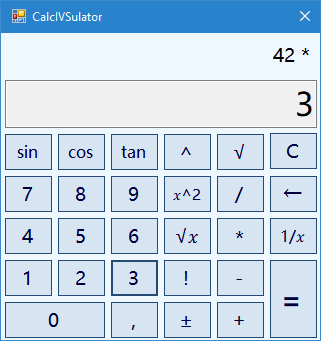
\includegraphics[width=0.75\linewidth]{calculator.PNG}}
            \annotatedFigureBox{0.01,0.0077}{0.9919,0.6176}{A}{0.01,0.31265}%bl
            \annotatedFigureBox{0.01,0.6176}{0.9919,0.7746}{B}{0.01,0.6961}%bl
            \annotatedFigureBox{0.01,0.7746}{0.9919,0.8875}{C}{0.01,0.83105}%bl
            \annotatedFigureBox{0.9,0.9}{1,1}{D}{0.885,0.95}%bl
        \end{annotatedFigure}
    \end{center}
    \vfill
    \newpage
    Uživatelské rozhraní je tvořeno čtyřmi častmi:

    \subsubsection{Klávesnice}
    Pomocí klávesnice lze zadat data do kalkulačky. Princip operace je vysvětlen vs sekci TODO. Funkce jednotlivých tlačítek je vysvětlena v sekci Funkce (TODO).

    \subsubsection{Výsledkový a zadávací displej}
    Zde se zobrazí výsledek Vaši operace nebo právě zadaný operand.

    \subsubsection{Displej s předchozí operací}
    Zde se zobrazí předchozí operand a operace, která je prováděna.

    \subsubsection{Ukončovací křížek}
    Pomocí křížku lze ukončit aplikaci.

    \subsection{Obecné používání}
    Proces pro většinu operací s kalkulačkou je následující. Doporučujeme si také přečíst sekci Zadávaní čísel (TODO).
    \begin{enumerate}
        \item Pomocí numerické klávesnice zadejte číslo prvního operandu.
        \item Vyberte požadovaou operaci pomocí klávesy funkce.
        \item Pokud je operace unární, zobrazí se výsledek, jinak pomocí numerické klávesnice zadejte druhý operand.
        \item Potvrďte druhý operand pomocí klávesy rovná se.
        \item Zobrazí se výsledek, nebo chybové hlášení; o chybových hlášeních Vás informuje ve sekci TODO.
    \end{enumerate}
    \subsection{Zadávání čísel}
\end{document}
